\section{\acs{approachname}}
\begin{frame}{\acs{approachname}}
    \begin{description}
    \item[\acs{approachname}] \acl{approachname}
    \end{description}
    
    \only<1>{
        \begin{figure}[htbp]
        \centering
            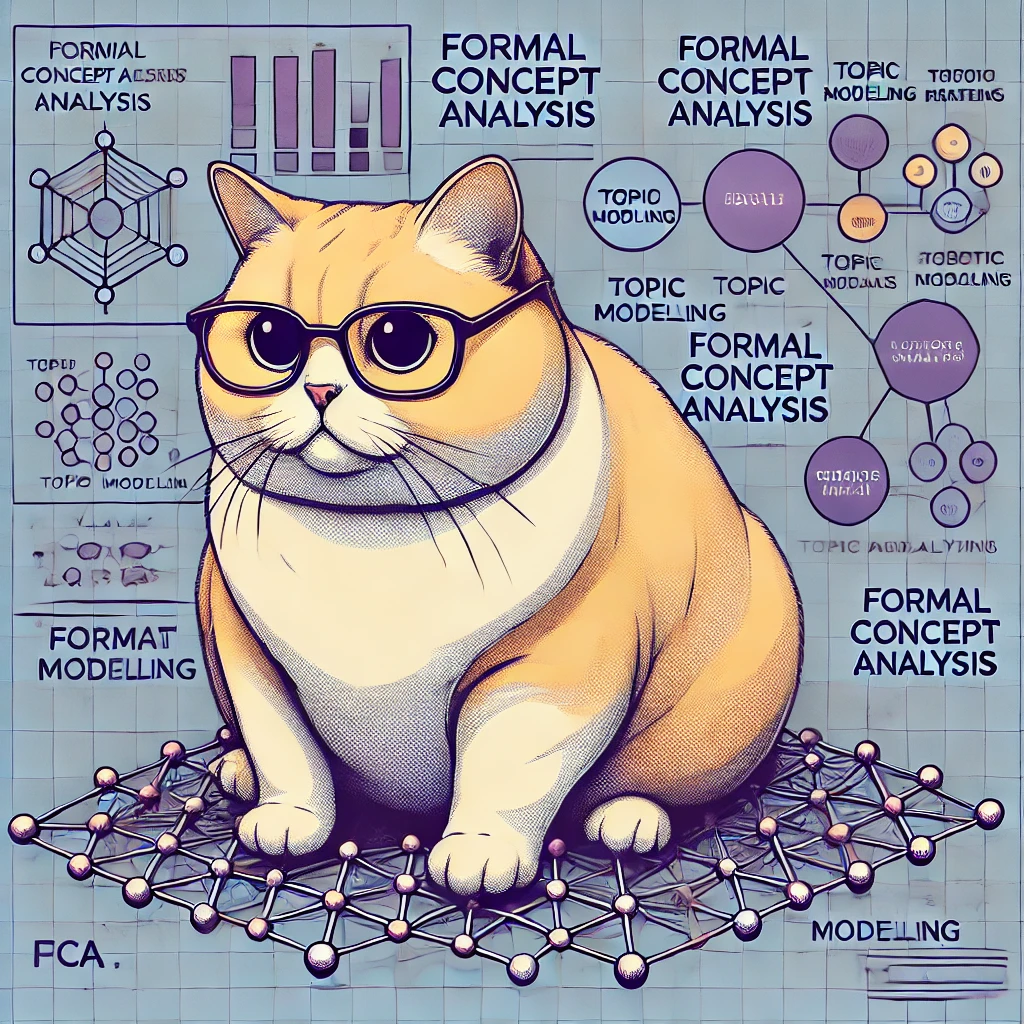
\includegraphics[height=0.6\textheight]{images/DALLE_2025_02_21_fat_cat.png}
        \label{fig:fat_cat}
    \end{figure}
    \begin{center}
        \scriptsize Image generated by DALLE (February 21, 2025)
    \end{center}
    }

    \only<2->{
        \begin{figure}[htbp]
        \centering
        \scalebox{0.9}{
            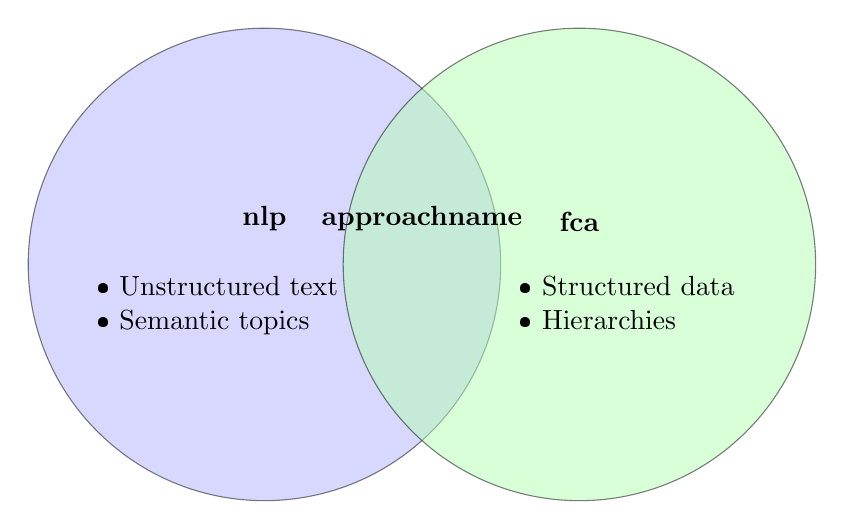
\begin{tikzpicture}
                 % Draw circles
                \draw[fill=blue!30, opacity=0.5] (-2,0) circle (3);
                \draw[fill=green!30, opacity=0.5] (2,0) circle (3);

                % Labels above circles
                \node[above] at (-2,0.3) {\textbf{\acs{nlp}}};
                \node[above] at (2,0.3) {\textbf{\acs{fca}}};
                \node[above] at (0,0.3) {\textbf{\acs{approachname}}};

                % NLP-only contributions (inside left circle, lower)
                \node[align=left] at (-2.6,-0.7) {
                    \textbullet\ Unstructured text\\
                    \textbullet\ Semantic topics\\
                    % \textbullet\ Statistical\\
                };

                % FCA-only contributions (inside right circle, lower)
                \node[align=left] at (2.6,-0.7) {
                    \textbullet\ Structured data\\
                    \textbullet\ Hierarchies\\
                    % \textbullet\ Deductive reasoning\\
                };
            \end{tikzpicture}
        }
        \label{fig:venn_nlp_fca}
    \end{figure}
    }

\end{frame}


\begin{frame}
    \begin{figure}
        \includesvg[width=\linewidth]{images/steps/overview_step3.svg}
    \end{figure}
\end{frame}


\begin{frame}{\acs{approachname}}
    \only<1>{
        \begin{figure}
            \includesvg[width=\linewidth]{images/topic_modeling_fca_2rows.svg}
        \end{figure}
    }
    
\end{frame}

\subsection{Text Extraction}
\begin{frame}{Text Extraction}
    \only<1>{
        \begin{figure}
            \includesvg[width=\linewidth]{images/steps_detail/topic_modeling_fca_2rows_step1.svg}
        \end{figure}
    }

    \only<2>{
        \begin{figure}
            \includesvg[width=\linewidth]{images/extract_text}
            \label{fig:extract_text}
        \end{figure}
        \begin{beamercolorbox}[center, wd=\linewidth, sep=1ex, rounded=true, shadow=true]{block body}
            {\small Appendix details: } 
            \hyperlink{supp:img_cap}{\beamergotobutton{Image Captioner}}
        \end{beamercolorbox}
    }
        
\end{frame}

\subsection{Topic Extraction}
\begin{frame}{\acs{approachname}}
    \begin{figure}
        \includesvg[width=\linewidth]{images/steps_detail/topic_modeling_fca_2rows_step2.svg}
    \end{figure}
\end{frame}

\begin{frame}{Topic Modeling}
    \begin{definition}
        Topic modeling is used for discovering latent semantic structure, usually referred to as topics, in a large collection of documents~\parencite{top2vec_2020}.
    \end{definition}
\end{frame}
\begin{frame}{Top2Vec~\parencite{top2vec_2020}}
    \includesvg[width=\linewidth]{images/Top2Vec}
    \begin{itemize}
        \item<2-> Words, documents and topics share vector space
        \item<2-> Multilingual \ac{use} 
        \begin{itemize}
            \item<2-> 16 languages
            \item<2-> 300-dimensional vector space
        \end{itemize}
        \item<3-> Dimensionality reduction to five dimensions
        \item<4-> Embeddings are clustered into topics
    \end{itemize}
\end{frame}

\subsection{Deriving the Directory-Topic Concept Lattice}
\begin{frame}{Directory-Topic Concept Lattice}
    \begin{textblock*}{3.8cm}(\paperwidth-3.9cm,0.2cm) % width + margin
        \only<1>{
            \includesvg[width=\linewidth]{images/steps_detail/topic_modeling_fca_2rows_step2.svg}
        }
        \only<3-4>{
            \includesvg[width=\linewidth]{images/steps_detail/topic_modeling_fca_2rows_step3.svg}
        }
        \only<5>{
            \includesvg[width=\linewidth]{images/steps_detail/topic_modeling_fca_2rows_step4.svg}
        }
    \end{textblock*}
    \only<1,3->{Assuming all documents are organized in directories.}
    \only<2>{
        \begin{figure}
            \includesvg[width=\linewidth]{images/steps_detail/topic_modeling_fca_2rows_step3.svg}
        \end{figure}
    }
    \begin{enumerate}
        \item <1,3-> Top 10 topics per document incl. relevance scores
        \item <3-> Compute threshold $\delta$ s.t. document-topic matrix density $< 0.1$
        \item <4-> $\mathcal{D}_\delta(i,j)=\left\{ \begin{array}{cl}
                        1 & \ \text{if } \ w_{i,j} \geq \delta, \\
                        0 & \ \text{else.}
                    \end{array} \right.$
        \item <5-> Compute iceberg lattice for each directory
    \end{enumerate}

    \only<3>{
        \centering
        \includesvg[width=0.6\linewidth]{images/Density_of_document_topic_incidence_matrix_altered}
    }

  \only<4>{
    \begin{center}
        \captionof{table}{Document-topic relation $\mathcal{D}_\delta$~\parencite{topic_modeling_2024}}
        \label{tab:doc-topic2}
        % \resizebox{\linewidth}{!}{%
            \begin{tabular}{|c|c|c|c|c|}
                \hline
                \diagbox{Documents}{Topics} & $t_1$ & $t_2$ & $\cdots$ & $t_n$ \\ \hline
                $d_1$ & $w_{1,1}$ & $w_{1,2}$ & $\cdots$ & $w_{1,n}$ \\ \hline
                $d_2$ & $w_{2,1}$ & $w_{2,2}$ & $\cdots$ & $w_{2,n}$ \\ \hline
                $\vdots$ & $\vdots$ & $\vdots$ & $\ddots$ & $\vdots$ \\ \hline
                $d_l$ & $w_{l,1}$ & $w_{l,2}$ & $\cdots$ & $w_{l,n}$ \\ \hline
            \end{tabular}
        % }
        \end{center}
    }

  

\end{frame}

\newcommand{\FormalConceptGraph}{%
\begin{tikzpicture}[
    concept/.style={
        circle, draw, minimum size=6mm, inner sep=1mm
    },
    level distance=15mm
]
    
    % Layer 0 (top)
    \node[concept] (n0) {};

    % Layer 1
    \node[concept, below left=15mm and 20mm of n0] (n1) {};
    \node[concept, below=15mm of n0] (n2) {};
    \node[concept, below right=15mm and 20mm of n0] (n3) {};

    % Layer 2
    \node[concept, below left=15mm and 15mm of n1] (n4) {};
    \node[concept, below right=15mm and 15mm of n1] (n5) {};
    \node[concept, below left=15mm and 15mm of n2] (n6) {};
    \node[concept, below right=15mm and 15mm of n2] (n7) {};
    \node[concept, below left=15mm and 15mm of n3] (n8) {};
    \node[concept, below right=15mm and 15mm of n3] (n9) {};

    % Layer 3
    \node[concept, below left=15mm and 10mm of n4] (n10) {};
    \node[concept, below=15mm and 10mm of n4] (n11) {};
    \node[concept, below left=15mm and 10mm of n5] (n12) {};
    \node[concept, below right=15mm and 10mm of n5] (n13) {};
    \node[concept, below left=15mm and 10mm of n6] (n14) {};
    \node[concept, below right=15mm and 10mm of n6] (n15) {};
    \node[concept, below left=15mm and 10mm of n7] (n16) {};
    \node[concept, below=15mm and 10mm of n9] (n17) {};
    \node[concept, below left=15mm and 10mm of n8] (n18) {};
    \node[concept, below right=15mm and 10mm of n8] (n19) {};
    \node[concept, below left=15mm and 10mm of n9] (n20) {};

    % Layer 4 (bottom)
    \node[concept, below=15mm of n10] (n22) {};
    \node[concept, below=15mm of n12] (n23) {};
    \node[concept, below=15mm of n14] (n24) {};
    \node[concept, below=15mm of n16] (n25) {};
    \node[concept, below=15mm of n18] (n26) {};
    \node[concept, below=15mm of n20] (n27) {};
    \node[concept, below=15mm of n11] (n28) {};
    \node[concept, below=15mm of n17] (n29) {};
    \node[concept, below=15mm of n19] (n30) {};

    % Single bottom node
    \node[concept] (n31) at ($ (n22)!0.5!(n30) + (0,-15mm) $) {};
    % \node[concept] (n31) at ($(n22)!0.5!(n30) - (0,15mm)$) {};
    % \node[concept, below=15mm of $(n22)!0.5!(n30)$] (n31) {};

    % Draw downward edges only
    \foreach \from/\to in {
        n0/n1, n0/n2, n0/n3,
        n1/n4, n1/n5, n2/n6, n2/n7, n3/n8, n3/n9,
        n4/n10, n4/n11, n5/n12, n5/n13, n6/n14, n6/n15, n7/n16, n7/n17, n8/n18, n8/n19, n9/n20, 
        n10/n22, n11/n25, n12/n23, n13/n28, n14/n24, n15/n22, n16/n25, n17/n29, n18/n26, n19/n30, n20/n27}
    {
        \draw (\from) -- (\to);
    }

    % Connect all bottom layer nodes to the single bottom node
    \foreach \n in {n22,n23,n24,n25,n26,n27,n28,n29,n30}
    {
        \draw (\n) -- (n31);
    }

\end{tikzpicture}%
}


\newcommand{\FormalConceptGraphColoured}{%
\begin{tikzpicture}[
    concept/.style={
        circle, draw, minimum size=6mm, inner sep=1mm
    },
    level distance=15mm
]

% Layer 0
\node[concept, fill=green!70] (n0) {};

% Layer 1
\node[concept, below left=15mm and 20mm of n0, fill=green!70] (n1) {};
\node[concept, below=15mm of n0, fill=green!70] (n2) {};
\node[concept, below right=15mm and 20mm of n0, fill=green!70] (n3) {};

   % Layer 2
    \node[concept, below left=15mm and 15mm of n1] (n4) {};
    \node[concept, below right=15mm and 15mm of n1] (n5) {};
    \node[concept, below left=15mm and 15mm of n2] (n6) {};
    \node[concept, below right=15mm and 15mm of n2] (n7) {};
    \node[concept, below left=15mm and 15mm of n3] (n8) {};
    \node[concept, below right=15mm and 15mm of n3] (n9) {};

    % Layer 3
    \node[concept, below left=15mm and 10mm of n4] (n10) {};
    \node[concept, below=15mm and 10mm of n4] (n11) {};
    \node[concept, below left=15mm and 10mm of n5] (n12) {};
    \node[concept, below right=15mm and 10mm of n5] (n13) {};
    \node[concept, below left=15mm and 10mm of n6] (n14) {};
    \node[concept, below right=15mm and 10mm of n6] (n15) {};
    \node[concept, below left=15mm and 10mm of n7] (n16) {};
    \node[concept, below=15mm and 10mm of n9] (n17) {};
    \node[concept, below left=15mm and 10mm of n8] (n18) {};
    \node[concept, below right=15mm and 10mm of n8] (n19) {};
    \node[concept, below left=15mm and 10mm of n9] (n20) {};

    % Layer 4 (bottom)
    \node[concept, below=15mm of n10] (n22) {};
    \node[concept, below=15mm of n12] (n23) {};
    \node[concept, below=15mm of n14] (n24) {};
    \node[concept, below=15mm of n16] (n25) {};
    \node[concept, below=15mm of n18] (n26) {};
    \node[concept, below=15mm of n20] (n27) {};
    \node[concept, below=15mm of n11] (n28) {};
    \node[concept, below=15mm of n17] (n29) {};
    \node[concept, below=15mm of n19] (n30) {};

    % Single bottom node
    \node[concept] (n31) at ($ (n22)!0.5!(n30) + (0,-15mm) $) {};
    % \node[concept] (n31) at ($(n22)!0.5!(n30) - (0,15mm)$) {};
    % \node[concept, below=15mm of $(n22)!0.5!(n30)$] (n31) {};

    % Draw downward edges only
    \foreach \from/\to in {
        n0/n1, n0/n2, n0/n3,
        n1/n4, n1/n5, n2/n6, n2/n7, n3/n8, n3/n9,
        n4/n10, n4/n11, n5/n12, n5/n13, n6/n14, n6/n15, n7/n16, n7/n17, n8/n18, n8/n19, n9/n20, 
        n10/n22, n11/n25, n12/n23, n13/n28, n14/n24, n15/n22, n16/n25, n17/n29, n18/n26, n19/n30, n20/n27}
    {
        \draw (\from) -- (\to);
    }

    % Connect all bottom layer nodes to the single bottom node
    \foreach \n in {n22,n23,n24,n25,n26,n27,n28,n29,n30}
    {
        \draw (\n) -- (n31);
    }


\end{tikzpicture}%
}





%%%%%%%%%%%%%%%%%%%%%%%%%%%%%%%%%%%%%%%%%%%%%%%
\begin{frame}{TITANIC~\cite{titanic_2002}}
\begin{columns}
\begin{column}{0.7\textwidth}
\begin{alertblock}{Problem} % with large datasets
The size of a concept lattice can grow exponentially with respect to the size of the context.
\end{alertblock}

\visible<2->{
    \begin{exampleblock}{Solution}
    Consider only top-level concepts.
    \end{exampleblock}
}
\end{column}

\begin{column}{0.25\textwidth}

\only<1>{
\begin{figure}[htbp]
    \centering
    \resizebox{\textwidth}{!}{\FormalConceptGraph}
    \caption{Concept lattice.}
    \label{fig:titanic_formal_concept_graph}
\end{figure}
}

\only<2->{
\begin{figure}[htbp]
    \centering
    \resizebox{\textwidth}{!}{\FormalConceptGraphColoured}
    \caption{Concept lattice.}
    \label{fig:titanic_formal_concept_graph_iceberg}
\end{figure}
}



\end{column}
\end{columns}
\end{frame}


\begin{frame}{TITANIC~\cite{titanic_2002}}
\begin{definition}
Support $supp(B) = \frac{\left| B' \right|}{\left| G \right|}$
\end{definition}


\begin{description}
    \item<2->[minimum support] $minsupp \in [0,1]$: Threshold below which attribute sets are not considered frequent
    \item <3-> [frequent attribute set] $B \subseteq M$: $supp(B) \ge minsupp$  % in $\mathbb{K}$ if
    \item <4-> [frequent concept] $(A, B)$: $B$ is frequent attribute set
\end{description}

    



\end{frame}

\begin{frame}{TITANIC~\cite{titanic_2002}}
\begin{columns}
    \begin{column}{0.7\textwidth}
        \begin{definition}
        The iceberg concept lattice of a context $\mathbb{K}$ comprises all frequent concepts.
        \end{definition}

        \visible<2->{
        \begin{description}
            \item[TITANIC] algorithm computes iceberg concept lattices.
        \end{description}
        % An iceberg concept lattice includes only the top-level concepts, specifically those corresponding to frequent attribute sets.
        }
    \end{column}
    \begin{column}{0.25\textwidth}
    \begin{figure}[htbp]
        \centering
        \resizebox{\textwidth}{!}{\FormalConceptGraphColoured}
        \caption{Iceberg concept lattice coloured.}
        \label{fig:titanic_formal_concept_graph_coloured}
    \end{figure}
    \end{column}
\end{columns}
\end{frame}

\begin{frame}{Directory-Topic Concept Lattice}
    \begin{textblock*}{3.8cm}(\paperwidth-3.9cm,0.2cm) % width + margin
        \only<1>{
            \includesvg[width=\linewidth]{images/steps_detail/topic_modeling_fca_2rows_step4.svg}
        }
        \only<2>{
            \includesvg[width=\linewidth]{images/steps_detail/topic_modeling_fca_2rows_step5.svg}
        }
        \only<3>{
            \includesvg[width=\linewidth]{images/steps_detail/topic_modeling_fca_2rows_step6.svg}
        }
    \end{textblock*}
    \only<1->{Assuming all documents are organized in directories.}

    \begin{enumerate}
        \item Top 10 topics per document incl. relevance scores
        \item Compute threshold $\delta$ s.t. document-topic matrix density $< 0.1$
        \item $\mathcal{D}_\delta(i,j)=\left\{ \begin{array}{cl}
                        1 & \ \text{if } \ w_{i,j} \geq \delta, \\
                        0 & \ \text{else.}
                    \end{array} \right.$
        \item Compute iceberg lattice for each directory
        \item <2-> Combine frequent topics across directories into directory-topic matrix
        \item[\rightarrowfill] <3-> Directory-topic context
    \end{enumerate}

      \only<1>{
        \begin{center}
            \resizebox{0.25\linewidth}{0.3\textheight}{%
                \FormalConceptGraphColoured
            }

            \vspace{0.5em}
            {\scriptsize Iceberg concept lattice coloured.}
        \end{center}
    }

    \only<2>{
        \begin{table}[t]
    \centering
    \caption{Weighted directory-topic relation.
        The weights $\tilde{w}_{i,j} \in \{0,1\}$ represent whether a topic $t_j$ is present in a directory $\hat{d}_i$.}
    \label{tab:dir-topic}
    \begin{tabular}{|c|c|c|c|c|}
        \hline
        \backslashbox{Directories}{Topics} & $t_1$             & $t_2$             &          & $t_n$             \\ \hline
        $\hat{d}_1$                        & $\tilde{w}_{1,1}$ & $\tilde{w}_{1,2}$ & $\cdots$ & $\tilde{w}_{1,n}$ \\ \hline
        $\hat{d}_2$                        & $\tilde{w}_{2,1}$ & $\tilde{w}_{2,2}$ & $\cdots$ & $\tilde{w}_{2,n}$ \\ \hline
        $\vdots$                           & $\vdots$          & $\vdots$          & $\ddots$ & $\vdots$          \\ \hline
        $\hat{d}_k$                        & $\tilde{w}_{k,1}$ & $\tilde{w}_{k,2}$ & $\cdots$ & $\tilde{w}_{k,n}$ \\ \hline
    \end{tabular}
\end{table}
    }
\end{frame}
